\documentclass[12pt,letterpaper]{article}
%\documentstyle[11pt]{article}
\usepackage[utf8]{inputenc}
\usepackage{amsmath}
\usepackage{xfrac}
\usepackage{amsfonts}
\usepackage{amssymb}
\usepackage[version = 3]{mhchem}
\usepackage{chemstyle}
%%For Table perhaps%%
%\usepackage{graphics}
\usepackage{graphicx}
\usepackage{epstopdf}
\usepackage{tabularx,ragged2e,booktabs,caption}
%\newcolumntype{C}[1]{>{\Centering}m{#1}}
\renewcommand\tabularxcolumn[1]{C{#1}}
\usepackage[left=1.5cm,right=1.5cm,top=1.5cm,bottom=1.5cm]{geometry}
\usepackage{subcaption} 
\usepackage{caption}
\usepackage[colorlinks]{hyperref}
\usepackage[svgnames]{xcolor}
\hypersetup{citecolor=DeepPink4}
\hypersetup{linkcolor=DarkRed}
\hypersetup{urlcolor=DarkBlue}
\usepackage{cleveref}
\usepackage{enumerate}

\begin{document}
\setlength{\parindent}{0cm} 


\frenchspacing

\title {\Large{\textbf{Midterm 1}}\\ \large{CENG 340--Introduction to Environmental Engineering\\
Instructor: Deborah Sills\\ \textbf{October 9, 2013}}}
\author {}
\date {}
\maketitle

\vspace{-1.5cm}

\textbf{\Large{Name:}}\\

As you work through the exam, please write down what you know (in equation form when possible), write down any questions you have (since I'm in Chicago).  And, please, \textbf{SHOW YOUR WORK!}

\begin{enumerate}

\item Alkalinity

\begin{enumerate}

\item \textbf{5pts} What is alkalinity (in words)?
\vspace{1in}

\item \textbf{5pts} Why is alkalinity important---Name one phenomena or system (natural or engineered) where alkalinity may play a role.

\vspace{1in}

\item \textbf{10pts} How many milliliters of a sulfuric acid (H$_2$SO$_4$) solution (concentration = 0.1 equivalents/liter) are needed to consume the alkalinity of 200 milliliters of lake water, which has an alkalinity of 250 mg/liter as CaCO$_3$?  Remember, sulfuric acid is a strong acid.

\vspace{4in}

\end{enumerate}



\item During a hydrofracking operation, the surfactant 2-butoxyethanol was accidentally released into a stream that is 2 meters deep.  The gas company---\emph{Energy Land}--- claims that no clean up is necessary, since 2-butoxyethanol will be broken down by microbes. However, because these microbes are aerobic, they also consume oxygen in proportion to the 2-butoxyethanol consumed, as shown in the following reaction:
\begin{align*}
\cee{C_6H_{12}O2\,  + \,  O_2\, \rightarrow \, CO_2 \, + \,  H_2O}
\end{align*}

\begin{enumerate}

\item \textbf{15 pts} Calculate the mass of 2-butoxyethanol (\textbf{in kg}) that spilled within an enclosed area of 10,000 m$^2$, if the dissolved oxygen (D.O.) concentration in this region was reduced by the microbes to 0.5 $\mathrm{\frac{mg\, O_2}{L}}$.  Assume that the normal ``background'' D.O. (outside the spill area) is 8 $\mathrm{\frac{mg\, O_2}{L}}$, and that all of the spilled 2-butoxyethanol remains in the aqueous phase (i.e., no water--gas or water--solid partitioning). 

\vspace{3in}

\item \textbf{10 pts} To avoid creating a ``Dead Zone'' (i.e., a region with very low dissolved oxygen levels), you have been asked to design an oxygen delivery system that will provide all of the oxygen needed by the microbes to break down the spilled surfactant.  Assume that 40 kg of 2-butoxyethanol is the total mass released in the spill (it's not).  Calculate the volume of a tank that would be required to store the total oxygen needed  to break down all of the pollutant.  Assume that the oxygen is stored under pressure with P = 50 atm, at a temperature, T = 25 $^0$C.

\vspace{4in}

\end{enumerate} 

\item \emph{For this problem, only use your calculator for the final steps of parts (c) and (e).}\\
To prevent future problems, the same gas company---\emph{Energy Land}--- hired you to design a reactor with a first-order reaction rate, that will remove 99 percent of the surfactant, 2-butoxyethanol, from frack flow-back water, at steady state.  You are considering a completely-mixed flow reactor (CMFR) and a plug-flow reactor (PFR). The design volumetric flow rate (Q), and the reaction rate coefficient (k) are known.  

\begin{enumerate}
\item \textbf{5 pts} For the CMFR, draw a schematic that includes an appropriate reactor, control volume, and all known and unknown variables.


\vspace{2in}

\item \textbf{10 pts} Write the \emph{complete} mass balance equation, including all variables. Then, clearly indicate which terms (if any) should not be considered for this problem.  Clearly state all assumptions made to simplify the mass balance equation.
\vspace{2in}


\item \textbf{10 pts} Solve the mass balance equation for the CMFR volume needed to achieve 99\% removal of 2-butoxyethanol in terms of volumetric flow rate and the reaction rate coefficient.

\vspace{4in}

\item \textbf{2 pts} For the PFR, draw a schematic that includes an appropriate reactor and all known and unknown variables.
\vspace{2in}

\item \textbf{10 pts} Use the equation we developed in class for a PFR (or write a complete mass balance equation) and solve for the volume needed to achieve 99\% removal of 2-butoxyethanol in terms of volumetric flow rate and the reaction rate coefficient.

\vspace{3in}


\item \textbf{5 pts} Provide a \textbf{brief} statement regarding the relative sizes of the reactors.  Should the volumes be the same or different?  Why?  

\pagebreak

\end{enumerate}

\item \textbf{13 pts}  A PFR and CMFR are in series as shown below.  The CMFR and PFR each has an initial concentration C$_0$ = 0.  And each reactor has the same volume, V.  A pulse input (mass = M) of a conservative material is introduced at the influent end of the PFR at t=0, and is immediately followed by a continuous flow, Q, with C=0. Sketch the concentration of the conservative material, C, vs. time in the effluent from the CMFR.   For your convenience, time intervals on the x-axis are given in multiples of the hydraulic retention time, $\mathrm{\theta = \frac{V}{Q}}$.

\begin{figure}
\centering
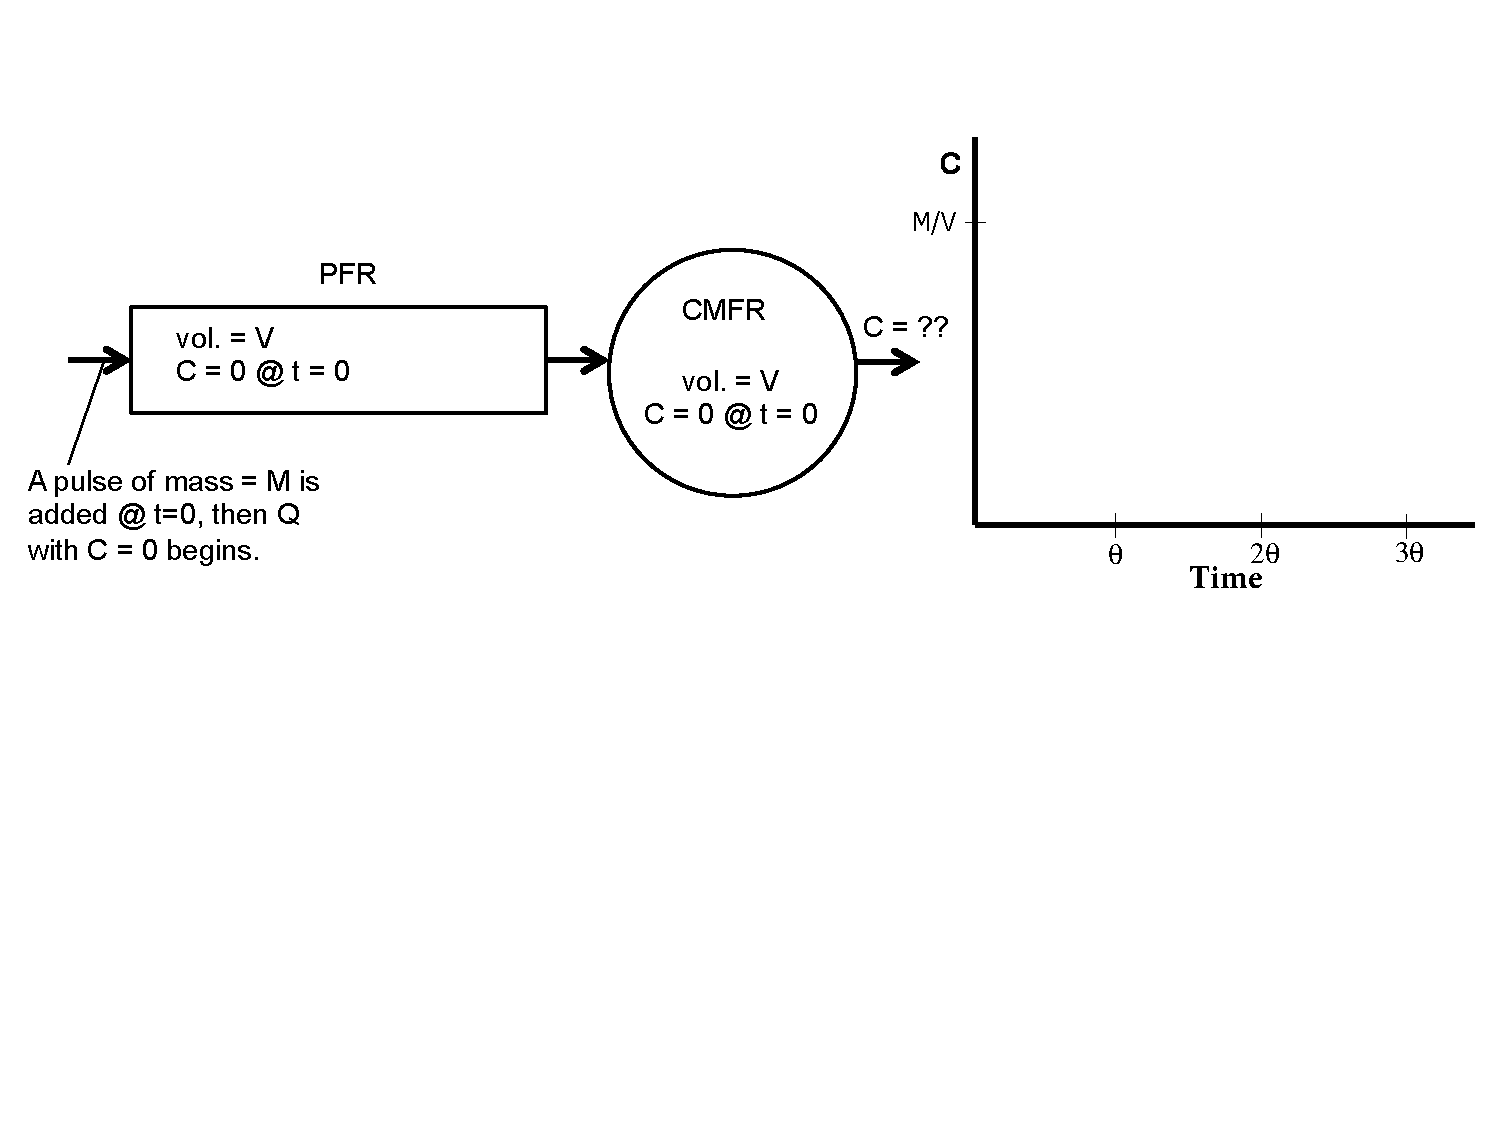
\includegraphics[width=1\textwidth]{pulse}
\end{figure}


\pagebreak

\item \textbf{13 pts} The parallel CMFR reactors shown below have their effluents mixed immediately as they exit each reactor. In addition, each reactor has an initial concentration C(0) = 0.  A continuous input to both CMFRs begins at t=0, and has a concentration of C = C$\mathrm{_{in}}$ of a conservative material.  Q and V for each reactor is the same.
\begin{enumerate}
\item Using a mass balance approach for one reactor develop an equation for C as a function of C$\mathrm{_{effluent}}$.
\vspace{3in}

\item Plot the expected concentration of the mixed effluents. 

\begin{figure}
\centering
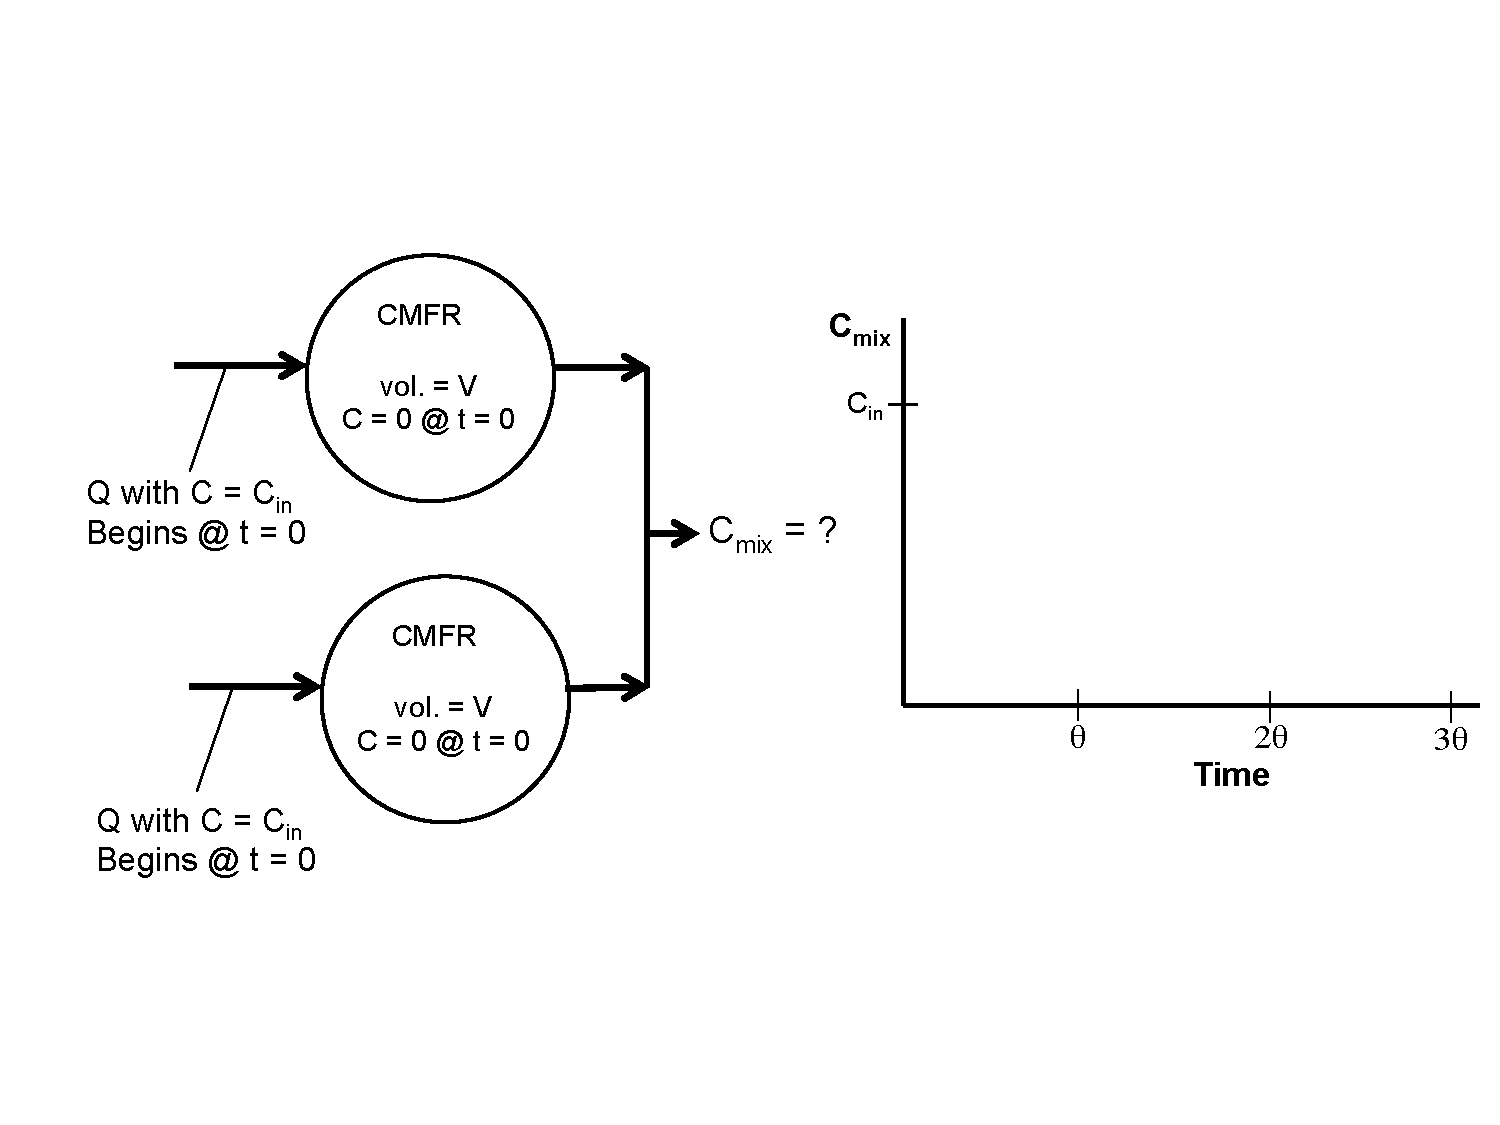
\includegraphics[width=1\textwidth]{two_cmfr}
\end{figure}

\end{enumerate}











\end{enumerate}
\end{document}